\documentclass[tikz,border=0pt]{standalone}
\usepackage[T1]{fontenc}
\usepackage{libertinus}
\usepackage{tikz}
\usetikzlibrary{calc,positioning,decorations.pathmorphing,shapes.geometric,fadings}

% Colors - Deep slate with neon cyan/green glow
\definecolor{DeepSlate}{RGB}{15,25,35}
\definecolor{MidSlate}{RGB}{25,40,55}
\definecolor{GlowCyan}{RGB}{0,220,180}
\definecolor{GlowGreen}{RGB}{80,255,160}
\definecolor{GlowBlue}{RGB}{60,180,255}
\definecolor{NodeCore}{RGB}{255,255,255}
\definecolor{WireGlow}{RGB}{0,200,170}
\definecolor{MetalLight}{RGB}{200,205,215}
\definecolor{MetalDark}{RGB}{140,150,165}
\definecolor{MetalMid}{RGB}{170,178,190}

\begin{document}
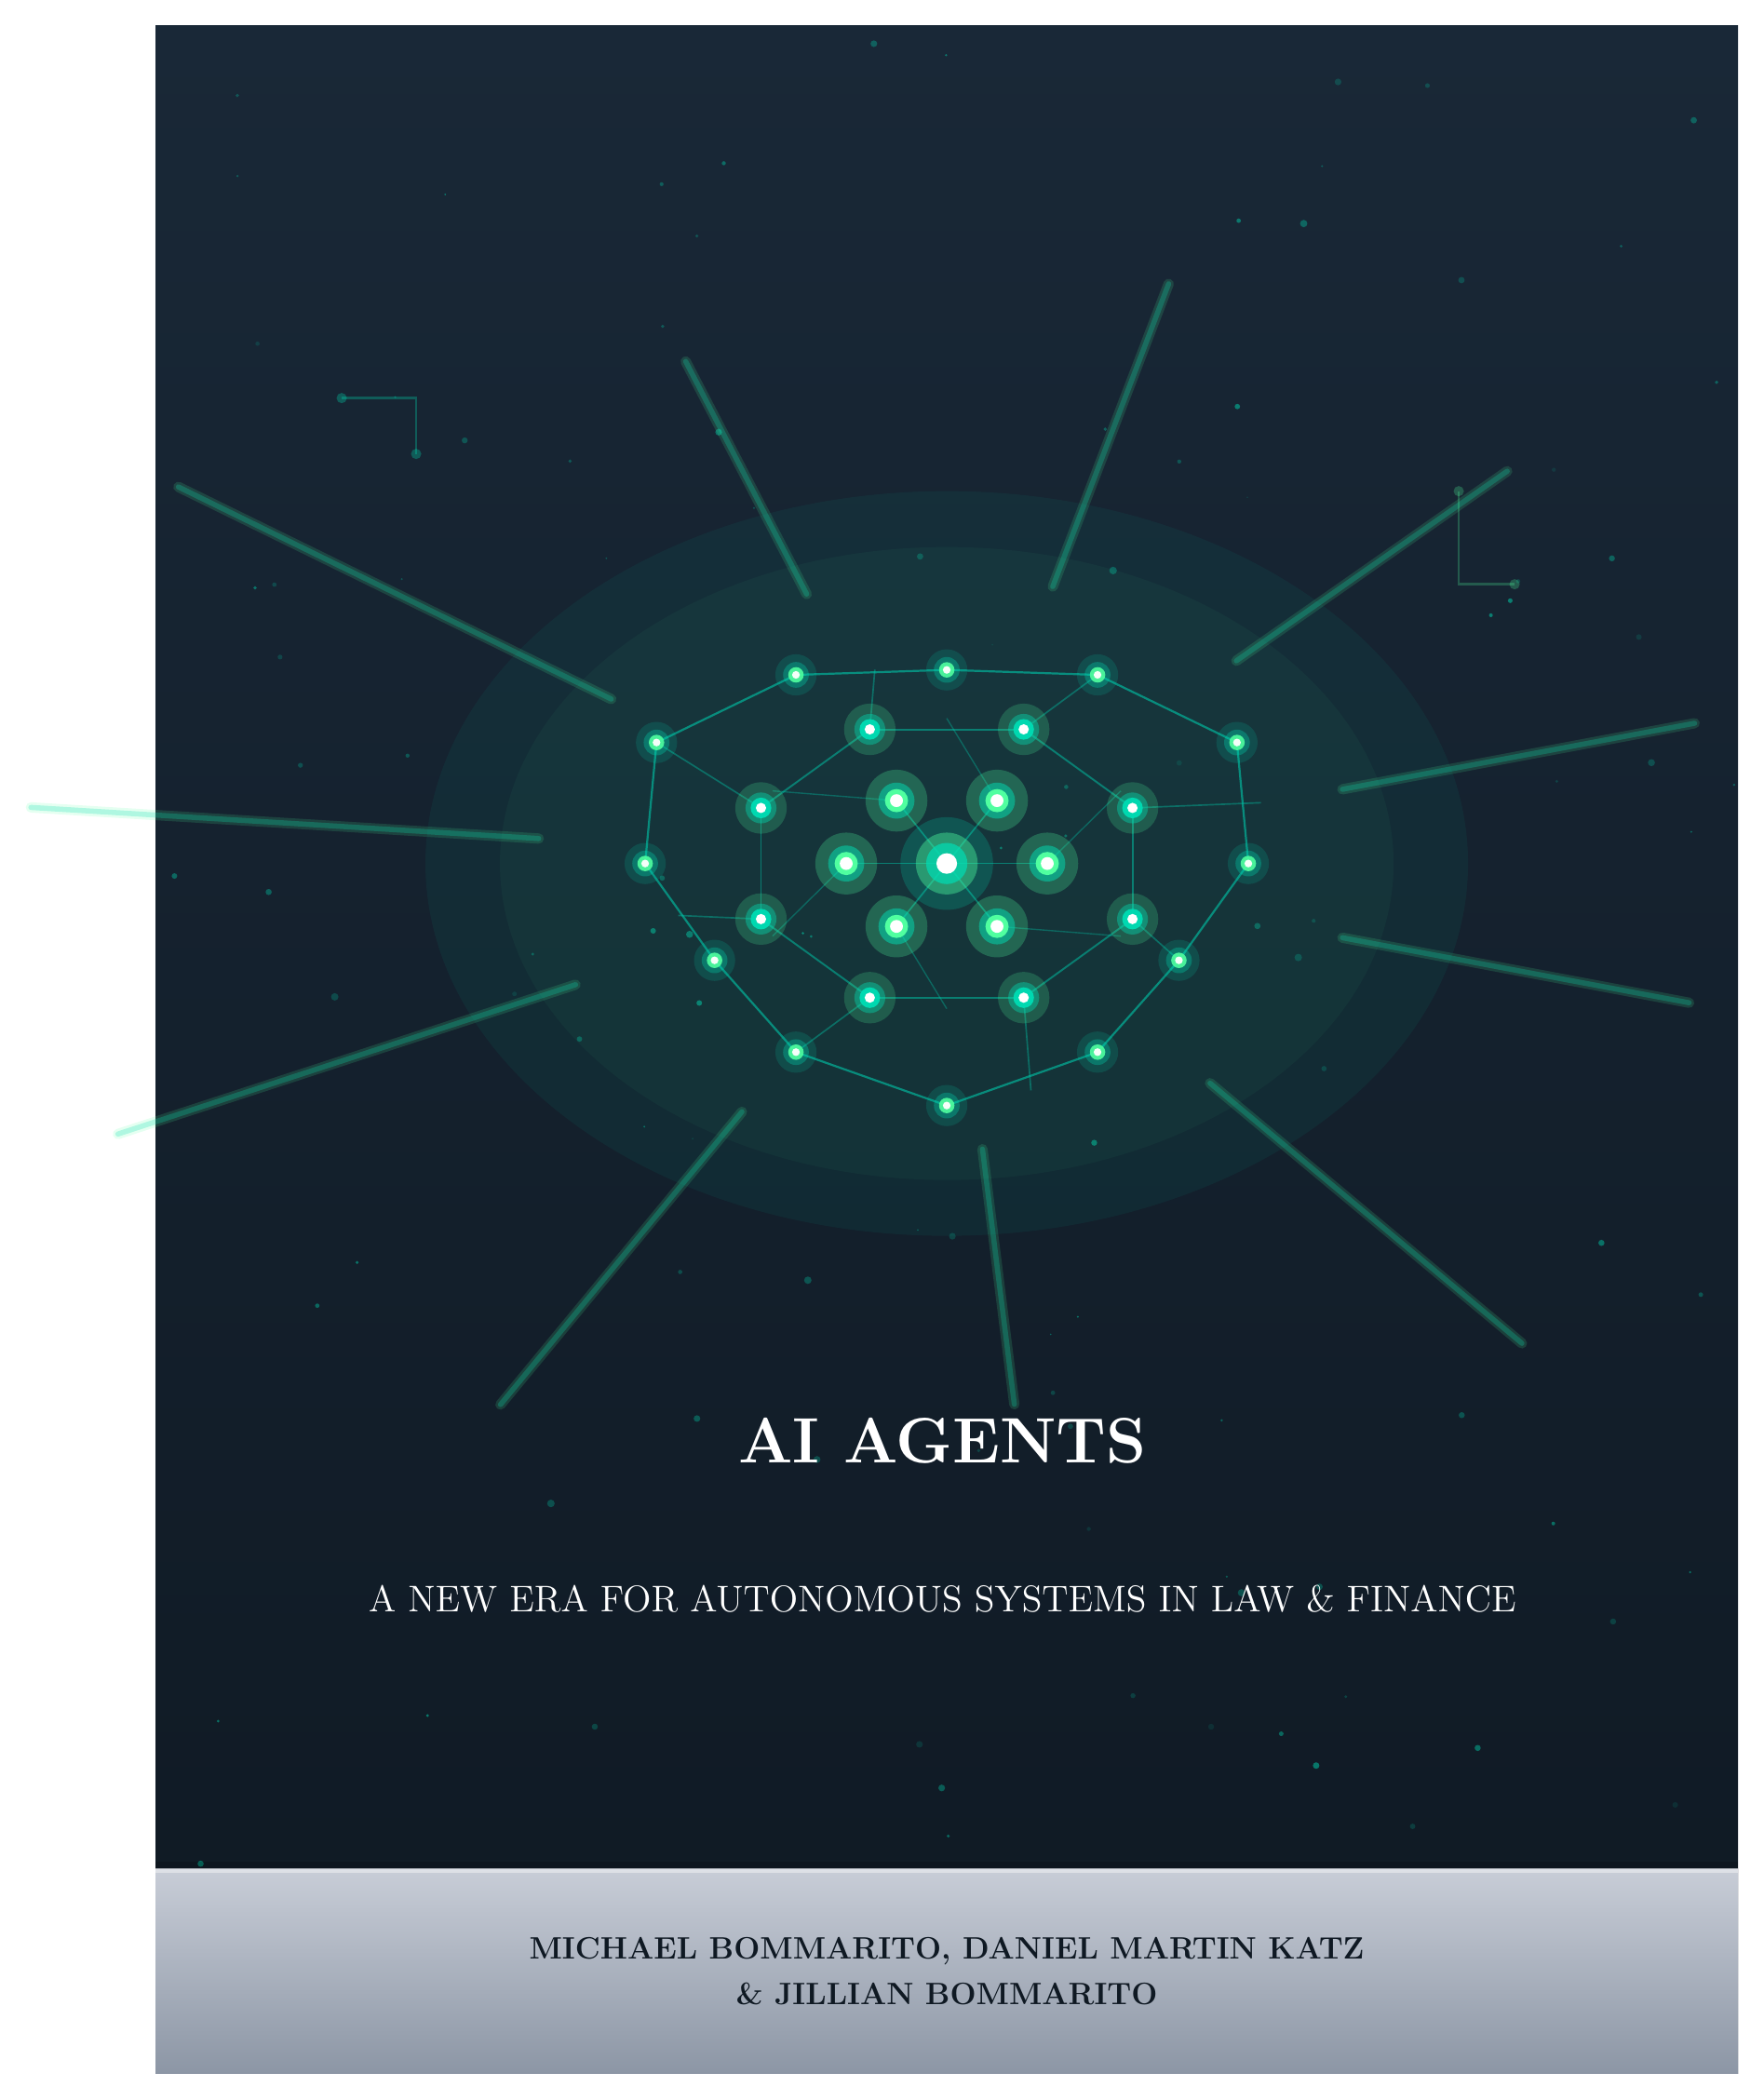
\begin{tikzpicture}

% Page dimensions (US Letter: 8.5 x 11 inches)
\def\pagewidth{8.5in}
\def\pageheight{11in}

% Background gradient - darker
\shade[top color=MidSlate, bottom color=DeepSlate]
  (0,0) rectangle (\pagewidth,\pageheight);

% Scattered particles throughout - creating depth
\foreach \i in {1,...,120} {
  \pgfmathsetmacro{\px}{random()*8.5}
  \pgfmathsetmacro{\py}{random()*11}
  \pgfmathsetmacro{\psize}{0.3 + random()*1.2}
  \pgfmathsetmacro{\popacity}{0.1 + random()*0.4}
  \fill[GlowCyan, opacity=\popacity] (\px in, \py in) circle (\psize pt);
}

% Motion blur streaks radiating from brain center
\begin{scope}[shift={(4.25in, 6.5in)}]
  \foreach \angle in {15, 45, 75, 110, 145, 175, 205, 240, 275, 310, 345} {
    \pgfmathsetmacro{\len}{1.8 + random()*1.2}
    \pgfmathsetmacro{\startdist}{2.2}
    \pgfmathsetmacro{\sx}{\startdist*cos(\angle)}
    \pgfmathsetmacro{\sy}{\startdist*sin(\angle)*0.7}
    \pgfmathsetmacro{\ex}{(\startdist+\len)*cos(\angle)}
    \pgfmathsetmacro{\ey}{(\startdist+\len)*sin(\angle)*0.7}
    \draw[GlowCyan, opacity=0.25, line width=2pt, line cap=round]
      (\sx in, \sy in) -- (\ex in, \ey in);
    \draw[GlowGreen, opacity=0.15, line width=4pt, line cap=round]
      (\sx in, \sy in) -- (\ex in, \ey in);
  }
\end{scope}

% 3D Wireframe brain structure
\begin{scope}[shift={(4.25in, 6.5in)}]

  % Background glow layers
  \fill[GlowCyan, opacity=0.06] (0,0) ellipse (2.8in and 2in);
  \fill[GlowGreen, opacity=0.04] (0,0) ellipse (2.4in and 1.7in);

  % Outer wireframe shell - brain boundary
  \foreach \i in {0,...,11} {
    \pgfmathsetmacro{\angle}{\i * 30}
    \pgfmathsetmacro{\nextangle}{(\i + 1) * 30}
    \pgfmathsetmacro{\r}{1.8 + 0.2*sin(\angle*3)}
    \pgfmathsetmacro{\rnext}{1.8 + 0.2*sin(\nextangle*3)}
    \pgfmathsetmacro{\x}{\r*cos(\angle)*0.9}
    \pgfmathsetmacro{\y}{\r*sin(\angle)*0.65}
    \pgfmathsetmacro{\xnext}{\rnext*cos(\nextangle)*0.9}
    \pgfmathsetmacro{\ynext}{\rnext*sin(\nextangle)*0.65}
    % Wireframe edges
    \draw[WireGlow, opacity=0.6, line width=0.8pt] (\x in, \y in) -- (\xnext in, \ynext in);
  }

  % Inner structure wireframe - creating depth
  \foreach \i in {0,...,7} {
    \pgfmathsetmacro{\angle}{\i * 45 + 22.5}
    \pgfmathsetmacro{\r}{1.2}
    \pgfmathsetmacro{\x}{\r*cos(\angle)*0.9}
    \pgfmathsetmacro{\y}{\r*sin(\angle)*0.65}
    % Connect to outer
    \pgfmathsetmacro{\outerangle}{\i * 45 + 15}
    \pgfmathsetmacro{\outerr}{1.8 + 0.2*sin(\outerangle*3)}
    \pgfmathsetmacro{\ox}{\outerr*cos(\outerangle)*0.9}
    \pgfmathsetmacro{\oy}{\outerr*sin(\outerangle)*0.65}
    \draw[WireGlow, opacity=0.4, line width=0.6pt] (\x in, \y in) -- (\ox in, \oy in);
  }

  % Inner wireframe ring
  \foreach \i in {0,...,7} {
    \pgfmathsetmacro{\angle}{\i * 45 + 22.5}
    \pgfmathsetmacro{\nextangle}{(\i + 1) * 45 + 22.5}
    \pgfmathsetmacro{\x}{1.2*cos(\angle)*0.9}
    \pgfmathsetmacro{\y}{1.2*sin(\angle)*0.65}
    \pgfmathsetmacro{\xnext}{1.2*cos(\nextangle)*0.9}
    \pgfmathsetmacro{\ynext}{1.2*sin(\nextangle)*0.65}
    \draw[WireGlow, opacity=0.5, line width=0.7pt] (\x in, \y in) -- (\xnext in, \ynext in);
  }

  % Core structure
  \foreach \i in {0,...,5} {
    \pgfmathsetmacro{\angle}{\i * 60}
    \pgfmathsetmacro{\x}{0.6*cos(\angle)*0.9}
    \pgfmathsetmacro{\y}{0.6*sin(\angle)*0.65}
    \draw[WireGlow, opacity=0.5, line width=0.6pt] (0,0) -- (\x in, \y in);
    % Connect to inner ring
    \pgfmathsetmacro{\innerangle}{\i * 60 + 30}
    \pgfmathsetmacro{\ix}{1.2*cos(\innerangle)*0.9}
    \pgfmathsetmacro{\iy}{1.2*sin(\innerangle)*0.65}
    \draw[WireGlow, opacity=0.35, line width=0.5pt] (\x in, \y in) -- (\ix in, \iy in);
  }

  % GLOWING NODES - Outer layer (largest glow)
  \foreach \i in {0,...,11} {
    \pgfmathsetmacro{\angle}{\i * 30}
    \pgfmathsetmacro{\r}{1.8 + 0.2*sin(\angle*3)}
    \pgfmathsetmacro{\x}{\r*cos(\angle)*0.9}
    \pgfmathsetmacro{\y}{\r*sin(\angle)*0.65}
    % Outer glow
    \fill[GlowCyan, opacity=0.15] (\x in, \y in) circle (8pt);
    \fill[GlowCyan, opacity=0.3] (\x in, \y in) circle (5pt);
    % Core
    \fill[GlowGreen, opacity=0.9] (\x in, \y in) circle (3pt);
    \fill[NodeCore, opacity=0.95] (\x in, \y in) circle (1.5pt);
  }

  % GLOWING NODES - Inner layer
  \foreach \i in {0,...,7} {
    \pgfmathsetmacro{\angle}{\i * 45 + 22.5}
    \pgfmathsetmacro{\x}{1.2*cos(\angle)*0.9}
    \pgfmathsetmacro{\y}{1.2*sin(\angle)*0.65}
    % Outer glow
    \fill[GlowGreen, opacity=0.2] (\x in, \y in) circle (10pt);
    \fill[GlowCyan, opacity=0.4] (\x in, \y in) circle (6pt);
    % Core
    \fill[GlowCyan, opacity=0.95] (\x in, \y in) circle (4pt);
    \fill[NodeCore] (\x in, \y in) circle (2pt);
  }

  % GLOWING NODES - Core layer (brightest)
  \foreach \i in {0,...,5} {
    \pgfmathsetmacro{\angle}{\i * 60}
    \pgfmathsetmacro{\x}{0.6*cos(\angle)*0.9}
    \pgfmathsetmacro{\y}{0.6*sin(\angle)*0.65}
    % Large glow
    \fill[GlowGreen, opacity=0.25] (\x in, \y in) circle (12pt);
    \fill[GlowCyan, opacity=0.5] (\x in, \y in) circle (7pt);
    % Core
    \fill[GlowGreen] (\x in, \y in) circle (4.5pt);
    \fill[NodeCore] (\x in, \y in) circle (2.5pt);
  }

  % Central hub - brightest node
  \fill[GlowCyan, opacity=0.2] (0,0) circle (18pt);
  \fill[GlowGreen, opacity=0.4] (0,0) circle (12pt);
  \fill[GlowCyan, opacity=0.7] (0,0) circle (8pt);
  \fill[NodeCore] (0,0) circle (4pt);

\end{scope}

% Small circuit-like elements in corners
\begin{scope}[shift={(1in, 9in)}, opacity=0.3]
  \draw[GlowCyan, line width=1pt] (0,0) -- (0.4in, 0) -- (0.4in, -0.3in);
  \fill[GlowCyan] (0,0) circle (2pt);
  \fill[GlowCyan] (0.4in, -0.3in) circle (2pt);
\end{scope}

\begin{scope}[shift={(7in, 8.5in)}, opacity=0.25]
  \draw[GlowGreen, line width=1pt] (0,0) -- (0, -0.5in) -- (0.3in, -0.5in);
  \fill[GlowGreen] (0,0) circle (2pt);
  \fill[GlowGreen] (0.3in, -0.5in) circle (2pt);
\end{scope}

% ============ TITLE SECTION ============

% Title with subtle glow effect
\node[anchor=center, align=center] at (4.25in, 3.4in) {
  {\fontsize{48}{56}\selectfont\bfseries\color{white}AI AGENTS}
};

% Subtitle
\node[anchor=center, align=center] at (4.25in, 2.55in) {
  {\fontsize{15}{20}\selectfont\color{white!85}A NEW ERA FOR AUTONOMOUS SYSTEMS IN LAW \& FINANCE}
};

% ============ METALLIC BAND AT BOTTOM ============

% Metallic gradient band
\shade[top color=MetalLight, bottom color=MetalDark]
  (0, 0) rectangle (\pagewidth, 1.1in);

% Highlight line at top of band
\fill[white, opacity=0.4] (0, 1.08in) rectangle (\pagewidth, 1.1in);

% Shadow line at top
\fill[black, opacity=0.15] (0, 1.1in) rectangle (\pagewidth, 1.14in);

% Author names on metallic band
\node[anchor=center, align=center] at (4.25in, 0.55in) {
  {\fontsize{13}{16}\selectfont\color{DeepSlate}\textbf{MICHAEL BOMMARITO, DANIEL MARTIN KATZ}}\\[0.08in]
  {\fontsize{13}{16}\selectfont\color{DeepSlate}\textbf{\& JILLIAN BOMMARITO}}
};

\end{tikzpicture}
\end{document}
